\chapter{The Smugglers}

Dantès had not been a day on board before he had a very clear idea of
the men with whom his lot had been cast. Without having been in the
school of the Abbé Faria, the worthy master of \textit{La Jeune Amélie} (the
name of the Genoese tartan) knew a smattering of all the tongues spoken
on the shores of that large lake called the Mediterranean, from the
Arabic to the Provençal, and this, while it spared him interpreters,
persons always troublesome and frequently indiscreet, gave him great
facilities of communication, either with the vessels he met at sea,
with the small boats sailing along the coast, or with the people
without name, country, or occupation, who are always seen on the quays
of seaports, and who live by hidden and mysterious means which we must
suppose to be a direct gift of Providence, as they have no visible
means of support. It is fair to assume that Dantès was on board a
smuggler.

At first the captain had received Dantès on board with a certain degree
of distrust. He was very well known to the customs officers of the
coast; and as there was between these worthies and himself a perpetual
battle of wits, he had at first thought that Dantès might be an
emissary of these industrious guardians of rights and duties, who
perhaps employed this ingenious means of learning some of the secrets
of his trade. But the skilful manner in which Dantès had handled the
lugger had entirely reassured him; and then, when he saw the light
plume of smoke floating above the bastion of the Château d’If, and
heard the distant report, he was instantly struck with the idea that he
had on board his vessel one whose coming and going, like that of kings,
was accompanied with salutes of artillery. This made him less uneasy,
it must be owned, than if the new-comer had proved to be a customs
officer; but this supposition also disappeared like the first, when he
beheld the perfect tranquillity of his recruit.

Edmond thus had the advantage of knowing what the owner was, without
the owner knowing who he was; and however the old sailor and his crew
tried to “pump” him, they extracted nothing more from him; he gave
accurate descriptions of Naples and Malta, which he knew as well as
Marseilles, and held stoutly to his first story. Thus the Genoese,
subtle as he was, was duped by Edmond, in whose favor his mild
demeanor, his nautical skill, and his admirable dissimulation, pleaded.
Moreover, it is possible that the Genoese was one of those shrewd
persons who know nothing but what they should know, and believe nothing
but what they should believe.

In this state of mutual understanding, they reached Leghorn. Here
Edmond was to undergo another trial; he was to find out whether he
could recognize himself, as he had not seen his own face for fourteen
years. He had preserved a tolerably good remembrance of what the youth
had been, and was now to find out what the man had become. His comrades
believed that his vow was fulfilled. As he had twenty times touched at
Leghorn, he remembered a barber in St. Ferdinand Street; he went there
to have his beard and hair cut. The barber gazed in amazement at this
man with the long, thick and black hair and beard, which gave his head
the appearance of one of Titian’s portraits. At this period it was not
the fashion to wear so large a beard and hair so long; now a barber
would only be surprised if a man gifted with such advantages should
consent voluntarily to deprive himself of them. The Leghorn barber said
nothing and went to work.

When the operation was concluded, and Edmond felt that his chin was
completely smooth, and his hair reduced to its usual length, he asked
for a looking-glass. He was now, as we have said, three-and-thirty
years of age, and his fourteen years’ imprisonment had produced a great
transformation in his appearance.

Dantès had entered the Château d’If with the round, open, smiling face
of a young and happy man, with whom the early paths of life have been
smooth, and who anticipates a future corresponding with his past. This
was now all changed. The oval face was lengthened, his smiling mouth
had assumed the firm and marked lines which betoken resolution; his
eyebrows were arched beneath a brow furrowed with thought; his eyes
were full of melancholy, and from their depths occasionally sparkled
gloomy fires of misanthropy and hatred; his complexion, so long kept
from the sun, had now that pale color which produces, when the features
are encircled with black hair, the aristocratic beauty of the man of
the north; the profound learning he had acquired had besides diffused
over his features a refined intellectual expression; and he had also
acquired, being naturally of a goodly stature, that vigor which a frame
possesses which has so long concentrated all its force within itself.

\begin{figure}[ht]
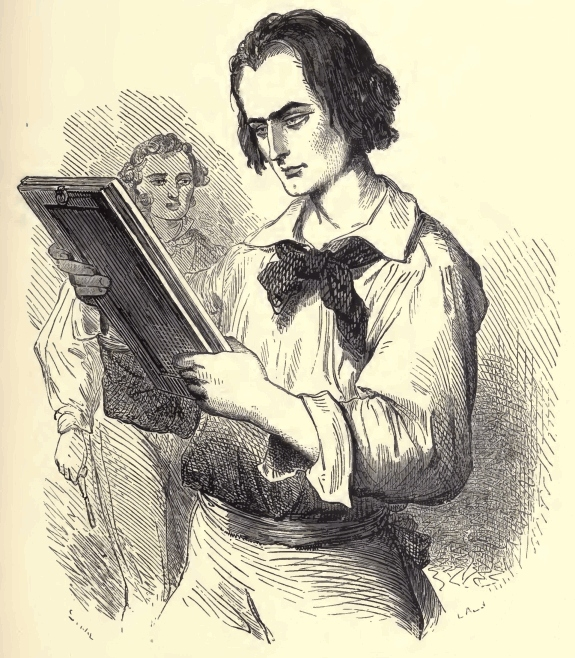
\includegraphics[width=\textwidth]{0283m.jpg}
\end{figure}

To the elegance of a nervous and slight form had succeeded the solidity
of a rounded and muscular figure. As to his voice, prayers, sobs, and
imprecations had changed it so that at times it was of a singularly
penetrating sweetness, and at others rough and almost hoarse.

Moreover, from being so long in twilight or darkness, his eyes had
acquired the faculty of distinguishing objects in the night, common to
the hyena and the wolf. Edmond smiled when he beheld himself; it was
impossible that his best friend—if, indeed, he had any friend
left—could recognize him; he could not recognize himself.

The master of \textit{La Jeune Amélie}, who was very desirous of retaining
amongst his crew a man of Edmond’s value, had offered to advance him
funds out of his future profits, which Edmond had accepted. His next
care on leaving the barber’s who had achieved his first metamorphosis
was to enter a shop and buy a complete sailor’s suit—a garb, as we all
know, very simple, and consisting of white trousers, a striped shirt,
and a cap.

It was in this costume, and bringing back to Jacopo the shirt and
trousers he had lent him, that Edmond reappeared before the captain of
the lugger, who had made him tell his story over and over again before
he could believe him, or recognize in the neat and trim sailor the man
with thick and matted beard, hair tangled with seaweed, and body
soaking in seabrine, whom he had picked up naked and nearly drowned.
Attracted by his prepossessing appearance, he renewed his offers of an
engagement to Dantès; but Dantès, who had his own projects, would not
agree for a longer time than three months.

\textit{La Jeune Amélie} had a very active crew, very obedient to their
captain, who lost as little time as possible. He had scarcely been a
week at Leghorn before the hold of his vessel was filled with printed
muslins, contraband cottons, English powder, and tobacco on which the
excise had forgotten to put its mark. The master was to get all this
out of Leghorn free of duties, and land it on the shores of Corsica,
where certain speculators undertook to forward the cargo to France.

They sailed; Edmond was again cleaving the azure sea which had been the
first horizon of his youth, and which he had so often dreamed of in
prison. He left Gorgone on his right and La Pianosa on his left, and
went towards the country of Paoli and Napoleon.

The next morning going on deck, as he always did at an early hour, the
patron found Dantès leaning against the bulwarks gazing with intense
earnestness at a pile of granite rocks, which the rising sun tinged
with rosy light. It was the Island of Monte Cristo.

\textit{La Jeune Amélie} left it three-quarters of a league to the larboard
and kept on for Corsica. Dantès thought, as they passed so closely to
the island whose name was so interesting to him, that he had only to
leap into the sea and in half an hour be at the promised land. But then
what could he do without instruments to discover his treasure, without
arms to defend himself? Besides, what would the sailors say? What would
the patron think? He must wait.

Fortunately, Dantès had learned how to wait; he had waited fourteen
years for his liberty, and now he was free he could wait at least six
months or a year for wealth. Would he not have accepted liberty without
riches if it had been offered to him? Besides, were not those riches
chimerical?—offspring of the brain of the poor Abbé Faria, had they not
died with him? It is true, the letter of the Cardinal Spada was
singularly circumstantial, and Dantès repeated it to himself, from one
end to the other, for he had not forgotten a word.

\begin{figure}[ht]
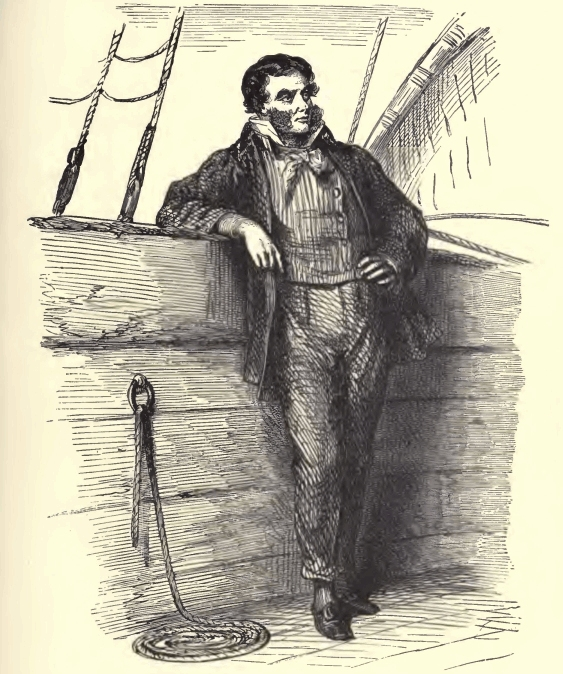
\includegraphics[width=\textwidth]{0285m.jpg}
\end{figure}

Evening came, and Edmond saw the island tinged with the shades of
twilight, and then disappear in the darkness from all eyes but his own,
for he, with vision accustomed to the gloom of a prison, continued to
behold it last of all, for he remained alone upon deck. The next morn
broke off the coast of Aleria; all day they coasted, and in the evening
saw fires lighted on land; the position of these was no doubt a signal
for landing, for a ship’s lantern was hung up at the mast-head instead
of the streamer, and they came to within a gunshot of the shore. Dantès
noticed that the captain of \textit{La Jeune Amélie} had, as he neared the
land, mounted two small culverins, which, without making much noise,
can throw a four ounce ball a thousand paces or so.

But on this occasion the precaution was superfluous, and everything
proceeded with the utmost smoothness and politeness. Four shallops came
off with very little noise alongside the lugger, which, no doubt, in
acknowledgement of the compliment, lowered her own shallop into the
sea, and the five boats worked so well that by two o’clock in the
morning all the cargo was out of \textit{La Jeune Amélie} and on \textit{terra
firma}. The same night, such a man of regularity was the patron of \textit{La
Jeune Amélie}, the profits were divided, and each man had a hundred
Tuscan livres, or about eighty francs.

But the voyage was not ended. They turned the bowsprit towards
Sardinia, where they intended to take in a cargo, which was to replace
what had been discharged. The second operation was as successful as the
first, \textit{La Jeune Amélie} was in luck. This new cargo was destined for
the coast of the Duchy of Lucca, and consisted almost entirely of
Havana cigars, sherry, and Malaga wines.

There they had a bit of a skirmish in getting rid of the duties; the
excise was, in truth, the everlasting enemy of the patron of \textit{La Jeune
Amélie}. A customs officer was laid low, and two sailors wounded;
Dantès was one of the latter, a ball having touched him in the left
shoulder. Dantès was almost glad of this affray, and almost pleased at
being wounded, for they were rude lessons which taught him with what
eye he could view danger, and with what endurance he could bear
suffering. He had contemplated danger with a smile, and when wounded
had exclaimed with the great philosopher, “Pain, thou art not an evil.”

He had, moreover, looked upon the customs officer wounded to death,
and, whether from heat of blood produced by the encounter, or the chill
of human sentiment, this sight had made but slight impression upon him.
Dantès was on the way he desired to follow, and was moving towards the
end he wished to achieve; his heart was in a fair way of petrifying in
his bosom. Jacopo, seeing him fall, had believed him killed, and
rushing towards him raised him up, and then attended to him with all
the kindness of a devoted comrade.

This world was not then so good as Doctor Pangloss believed it, neither
was it so wicked as Dantès thought it, since this man, who had nothing
to expect from his comrade but the inheritance of his share of the
prize-money, manifested so much sorrow when he saw him fall.
Fortunately, as we have said, Edmond was only wounded, and with certain
herbs gathered at certain seasons, and sold to the smugglers by the old
Sardinian women, the wound soon closed. Edmond then resolved to try
Jacopo, and offered him in return for his attention a share of his
prize-money, but Jacopo refused it indignantly.

As a result of the sympathetic devotion which Jacopo had from the first
bestowed on Edmond, the latter was moved to a certain degree of
affection. But this sufficed for Jacopo, who instinctively felt that
Edmond had a right to superiority of position—a superiority which
Edmond had concealed from all others. And from this time the kindness
which Edmond showed him was enough for the brave seaman.

Then in the long days on board ship, when the vessel, gliding on with
security over the azure sea, required no care but the hand of the
helmsman, thanks to the favorable winds that swelled her sails, Edmond,
with a chart in his hand, became the instructor of Jacopo, as the poor
Abbé Faria had been his tutor. He pointed out to him the bearings of
the coast, explained to him the variations of the compass, and taught
him to read in that vast book opened over our heads which they call
heaven, and where God writes in azure with letters of diamonds.

And when Jacopo inquired of him, “What is the use of teaching all these
things to a poor sailor like me?” Edmond replied, “Who knows? You may
one day be the captain of a vessel. Your fellow-countryman, Bonaparte,
became emperor.” We had forgotten to say that Jacopo was a Corsican.

Two months and a half elapsed in these trips, and Edmond had become as
skilful a coaster as he had been a hardy seaman; he had formed an
acquaintance with all the smugglers on the coast, and learned all the
Masonic signs by which these half pirates recognize each other. He had
passed and re-passed his Island of Monte Cristo twenty times, but not
once had he found an opportunity of landing there.

He then formed a resolution. As soon as his engagement with the patron
of \textit{La Jeune Amélie} ended, he would hire a small vessel on his own
account—for in his several voyages he had amassed a hundred
piastres—and under some pretext land at the Island of Monte Cristo.
Then he would be free to make his researches, not perhaps entirely at
liberty, for he would be doubtless watched by those who accompanied
him. But in this world we must risk something. Prison had made Edmond
prudent, and he was desirous of running no risk whatever. But in vain
did he rack his imagination; fertile as it was, he could not devise any
plan for reaching the island without companionship.

Dantès was tossed about on these doubts and wishes, when the patron,
who had great confidence in him, and was very desirous of retaining him
in his service, took him by the arm one evening and led him to a tavern
on the Via del’ Oglio, where the leading smugglers of Leghorn used to
congregate and discuss affairs connected with their trade. Already
Dantès had visited this maritime Bourse two or three times, and seeing
all these hardy free-traders, who supplied the whole coast for nearly
two hundred leagues in extent, he had asked himself what power might
not that man attain who should give the impulse of his will to all
these contrary and diverging minds. This time it was a great matter
that was under discussion, connected with a vessel laden with Turkey
carpets, stuffs of the Levant, and cashmeres. It was necessary to find
some neutral ground on which an exchange could be made, and then to try
and land these goods on the coast of France. If the venture was
successful the profit would be enormous, there would be a gain of fifty
or sixty piastres each for the crew.

The patron of \textit{La Jeune Amélie} proposed as a place of landing the
Island of Monte Cristo, which being completely deserted, and having
neither soldiers nor revenue officers, seemed to have been placed in
the midst of the ocean since the time of the heathen Olympus by
Mercury, the god of merchants and robbers, classes of mankind which we
in modern times have separated if not made distinct, but which
antiquity appears to have included in the same category.

At the mention of Monte Cristo Dantès started with joy; he rose to
conceal his emotion, and took a turn around the smoky tavern, where all
the languages of the known world were jumbled in a \textit{lingua franca}.

When he again joined the two persons who had been discussing the
matter, it had been decided that they should touch at Monte Cristo and
set out on the following night. Edmond, being consulted, was of opinion
that the island afforded every possible security, and that great
enterprises to be well done should be done quickly.

Nothing then was altered in the plan, and orders were given to get
under weigh next night, and, wind and weather permitting, to make the
neutral island by the following day.

\begin{figure}[ht]
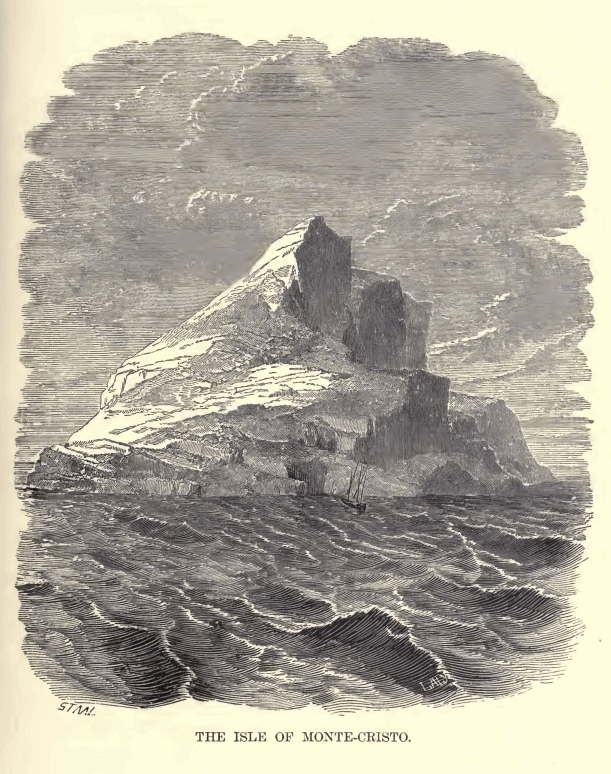
\includegraphics[width=\textwidth]{0289m.jpg}
\end{figure}
